\section{Filtro}

\begin{figure}[ht!]
\begin{center}
	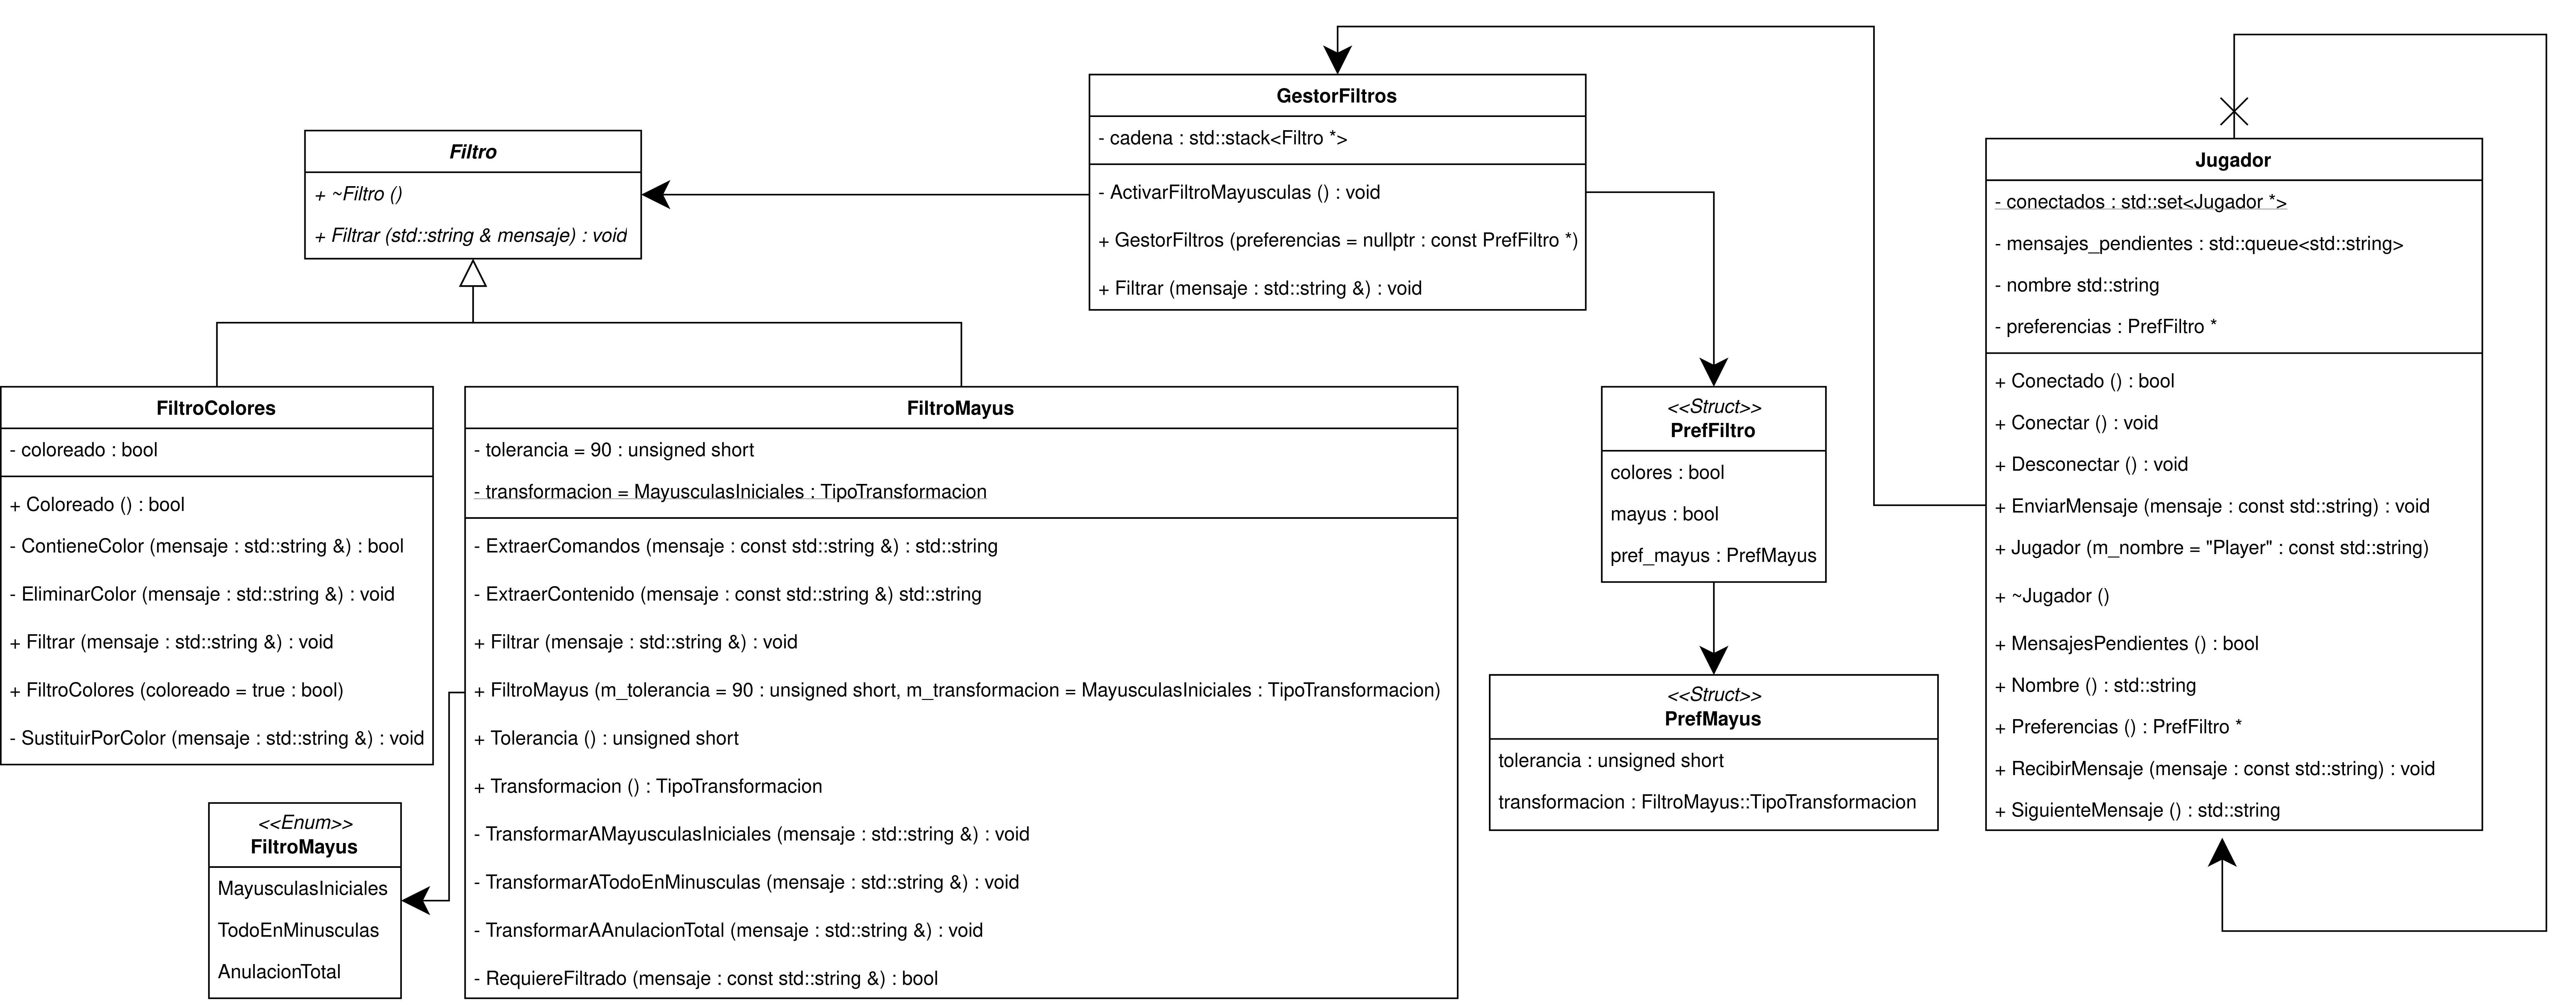
\includegraphics[scale=0.06]{DiagramaFiltro}
\end{center}
\caption{Diagrama UML de la aplicación del patrón \textit{Filtro}.}
\end{figure}

Nuestra aplicación del patrón \textit{Filtro} consiste en una demo del sistema de chat entre los jugadores de \textit{CaveArt}.
Cuando un jugador envía un mensaje, hace una transmisión a todos los jugadores conectados al chat para que todos reciban el mensaje.
Cada jugador tiene unas preferencias de chat propias, de forma que un jugador podrá decidir si quiere filtrar unos elementos u otros.

Las preferencias se almacenan en un \texttt{struct PrefFiltro} y son las siguientes:

\begin{itemize}
	\item\texttt{bool colores}\textbf{:}
		Filtrar o no los colores.
	\item\texttt{bool mayus}\textbf{:}
		Filtrar o no las mayúsculas.
	\item\texttt{struct PrefMayus}\textbf{:}
		Preferencias de filtrado de mayúsculas.
		\begin{itemize}
			\item\texttt{unsigned short tolerancia}\textbf{:}
				Porcentaje de caracteres alfebéticos en mayúsculas necesario para realizar el filtrado.
			\item\texttt{FiltroMayus::TipoTransformacion transformacion}\textbf{:}
				Transformación a aplicar a las mayúsculas.
		\end{itemize}
\end{itemize}

El filtrado de mayúsculas puede hacerse mediante tres trasnformaciones en orden de severidad:

\begin{itemize}
	\item\texttt{TipoTransformacion::MayusculasIniciales}
		Dejar en mayúsculas la primera letra de cada palabra.
	\item\texttt{TipoTransformacion::TodoEnMinusculas}
		No dejar ninguna mayúscula.
	\item\texttt{TipoTransformacion::AnulacionTotal}
		Eliminar el mensaje y no recibirlo
\end{itemize}

El filtrado de colores permite al jugador escribir un comando con la sintaxis \texttt{color:mensaje} para que los jugadores que filtran los colores lo reciban de ese color.
Se permiten los colores \texttt{red}, \texttt{green}, \texttt{yellow}, \texttt{blue}, \texttt{magenta} y \texttt{cyan}.

El \texttt{GestorFiltros} implementa la cadena de filtros como un \texttt{std::stack<Filtro *>}, simplificando así la estructura de clases.
Esto lo hacemos porque la cadena de filtros al final es una lista de filtros que se ejecutan detrás de otro, por lo que podemos utilizar cualquier estructura que respete el orden que queremos utilizar a la hora de filtrar (tanto \texttt{std::set<Filtro *>} como \texttt{std::vector<Filtro *>} habrían funcionado también).
En lugar de delegar la responsabilidad de ejecutar la cadena a ella mismo, se la damos al gestor, que lo único que tiene que hacer es ejecutar el último filtro y destruirlo hasta que la cadena esté vacía:

\begin{lstlisting}[language=C++]
void GestorFiltros :: Filtrar (std::string & mensaje) noexcept
{
	while (!cadena.empty())
	{
		cadena.top()->Filtrar(mensaje);
		delete cadena.top();
		cadena.pop();
	}
}
\end{lstlisting}
